\documentclass{article}

% Language setting
% Replace `english' with e.g. `spanish' to change the document language
\usepackage[english, russian]{babel}

% Set page size and margins
% Replace `letterpaper' with `a4paper' for UK/EU standard size
\usepackage[letterpaper,top=1cm,bottom=1.5cm,left=1cm,right=1cm,marginparwidth=1cm]{geometry}

%  Русский язык
\usepackage[T2A]{fontenc}			
\usepackage[utf8]{inputenc}	

%Красная строка для первого абзаца
\usepackage{indentfirst}

%Готические буквы
\usepackage{amssymb}

% Useful packages
\usepackage{amsmath}
\usepackage{siunitx}
\usepackage{accents}
\usepackage{graphicx}
\usepackage{subcaption}
\usepackage{caption}
\usepackage[colorlinks=true, allcolors=blue]{hyperref}
\usepackage{gensymb}
\usepackage{float}
\restylefloat{figure}  % Отключить float для всех figure
\restylefloat{table}   % Отключить float для всех table
\usepackage{pgfplots}
\pgfplotsset{compat=1.18}
\usepackage{geometry}
\geometry{a4paper, left=10mm, right=10mm, top=10mm, bottom=20mm}

\title{\textbf{Вопрос по выбору "Сканер поля антенн"}}
\author{Работу выполнили Юровская Дарья и Паламарчук Алексей, группа Б04-406}
\date{6 мая 2026 г}

\begin{document}
\maketitle

\section*{Аннотация}

\textbf{Цель}: собрать устройство (сканер), позволяющее получать карту фаз и амплитуд ближнего поля различных излучателей, а также преобразования этиого поля в дальнее.

Для достижения данной цели нам необходимо выполнить следующие задачи:

\begin{itemize}
    \item разработать схему нужного устройства;
    \item изготовить сканер;
    \item подготовить необходимое программное обеспечение, выполняющее сканирование ближнего поля по заданной площади поверхности;
    \item составить решатор, который бы отображал получившиеся карты амплитду и фаз, диаграмму направленности изучаемого излучателя;
    \item с помощью собранного устройства провести некоторые эксперименты по изучении дифракции на СВЧ-волнах;
    \item оценить корректность полученных результатов и правильность сборки сканера.
\end{itemize}
\section*{Схема экспериментальной установки}

Необходимо создать устройство, выполняющее задачи сканера: получение информации об амплитуде и фазе электромагнитного поля некоторой антенны в каждой точке некоторой площади. Но так как невозможно создать прибор, который би непрерывно снимал показания, то нужно, чтобы он делал измерения с некоторым шагом, который бы экспериментатор мог регулировать. Другими словами, необходимо создать сетку сканирования, в узлах которых будут производиться измерения.

В качестве прототипа использовался сканер для 3D-печати (см. рис. 1).

\begin{figure}[H]
    \centering
    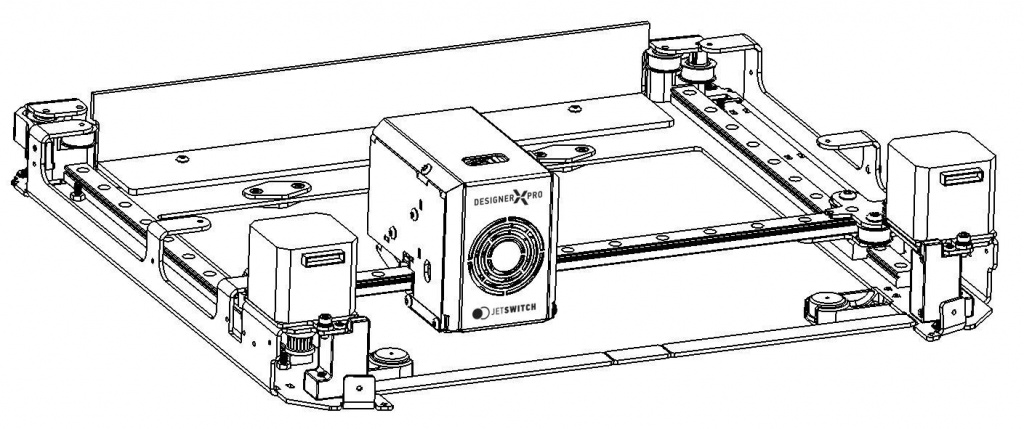
\includegraphics[width=0.75\linewidth]{Рис. 1.png}
    \caption{Схема принтера для 3D-печати}
    \label{fig:placeholder}
\end{figure}

Каркас установки представляет собой четыре скреплённых между собой алюминиевых профиля, размещённых на несколько укороченных таких же алюминиемых профилях. Перпендикулярно двум параллельным линиям, которые образуют профили, расположена другая такая же алюмириевая балка. На ней же будет установлена каретка с зондом, который, перемещаясь по всей сканируемой площади, делая измерения.

Движение алюминиевых профилей осуществляется при помощи шаговых моторов и зубчатых ремней. Два из них установлены на двух пареллельных балках -- они реализуют движение перпенудикулярному им профилю, а также движение зонда по оси $Ox$. Ещё один мотор расположен на подвижной балке -- он выполняет передвижение зонда вдоль оси $Oy$.

Каретка, на которой расположен зонд, выполнена в виде небольшой подложки, где и закрепляется измерительная антенна, а также небольшой конструкции для крепления провода.

Измерительная чвасть представляет собой зонд, соединённый коаксиальным кабелем с векторным анализатором цепей, второй коаксиальный кабель которого подключается к самой измеряемой антенне. Данные с векторного анализатора направляется на компьютер, где информация о получаемой амплитуде и фазе в конкретной точке сканируемой площади обрабытвается и строится карта распределения этих параметров. Кроме того, зная распределения амплитуды и фазы в ближнем поле, при помощи пространственного преобразования Фурье или метода Стреттона-Чу.
\end{document}